\documentclass{article}[11pt]

\usepackage{amsmath}
\usepackage{amssymb}
\usepackage{nicefrac}

\usepackage{pdflscape}

\usepackage{upgreek}

\usepackage{bashful}

% No intendation
\setlength\parindent{0pt}

\usepackage{hyperref}

\usepackage{siunitx}
\sisetup{
  per-mode=fraction,
  fraction-function=\tfrac
}

\usepackage{listings}
  \lstset{
    basicstyle=\ttfamily,
    escapeinside=||,
    xleftmargin=1cm
  }

\usepackage{float}

\usepackage{longtable}

\usepackage{multirow}

\usepackage{tikz}
  \usetikzlibrary{patterns}
  \usetikzlibrary{arrows.meta}
  \usetikzlibrary{shapes.misc}
  \usetikzlibrary{calc}

\usepackage{pgfplots}

\usepackage{cleveref}
\crefmultiformat{equation}{(#2#1#3)}{ and~(#2#1#3)}{, (#2#1#3)}{ and~(#2#1#3)}


\usepackage{acronym}
\usepackage[acronym,nonumberlist]{glossaries}
\glsdisablehyper
\makeglossaries
\newacronym{spice}{SPICE}{Simulation Program with Integrated Circuit Emphasis}
\newacronym{lef}{LEF}{Library Exchange Format}
\newacronym{dft}{DFT}{Discrete Fourier Transform}
\newacronym{dtft}{DTFT}{Discrete-Time Fourier Transform}
\newacronym{fft}{FFT}{Fast Fourier Transform}
\newacronym{mosfet}{MOSFET}{Metal–Oxide–Semiconductor Field-Effect Transistor}
\newacronym{clm}{CLM}{Channel Length Modulation}
\newacronym{de}{DE}{differential equation}
\newacronym{soi}{SOI}{silicon-on-insulator}
\newacronym{ldo}{LDO}{low-dropout regulator}
\newacronym{ota}{OTA}{operational-transconductance amplifier}
\newacronym{ofa}{OFA}{operational-floating amplifier}

% literature
\usepackage[ backend=biber
           , isbn=true
           , sorting=none
           , style=ieee
           ]{biblatex}
\addbibresource{./../../literature.bib}

% definitions
\def \whatis       {Notes}
\def \title        {Fuubar}

\def \author       {Matthias Schweikardt}

\def \authorMail   {mschweikardt@posteo.de}

\def \authorGithub {mschweikardt}

\def \license      {CC BY-SA 4.0}
\def \licenseUrl   {https://creativecommons.org/licenses/by-sa/4.0/}

\def \date         {nodate}

\def \pdfurl       {https://mschweikardt.github.io/ee-notes/%
\bash[stdout]
IFS=/ 
var=($PWD)
echo ${var[-1]}
\END%
.pdf
}
\def \srcurl       {srcurl}


% Customize footer and header of document
\usepackage{fancyhdr}

% Access last page number
\usepackage{lastpage}

% Access last page number
\usepackage[thinc]{esdiff}

% Physics
\usepackage{physics}

% Comment environment
\usepackage{comment}

% Subcaptions
\usepackage{subcaption}

% Thicker lines in tables
\usepackage{booktabs}

% Indentation in footnote
\makeatletter
\renewcommand\@makefntext[1]{\leftskip=2em\hskip-0.5em\@makefnmark#1}
\makeatother         

% qty with the siunitx definition
\AtBeginDocument{\RenewCommandCopy\qty\SI}

% TikZ compatibility
\pgfplotsset{compat=1.18}


\makeatletter
\pgfmathdeclarefunction{myatan2}{2}{%
\begingroup%
  \pgfmathfloattofixed{#1}\edef\tempa{\pgfmathresult}%
  \pgfmathfloattofixed{#2}%
  \pgfkeys{pgf/fpu=false}%
  \pgfmathparse{atan2(\tempa,\pgfmathresult)}\pgfkeys{/pgf/fpu}%
  \pgfmathfloatparsenumber{\pgfmathresult}%
  \pgfmath@smuggleone\pgfmathresult%
\endgroup
}
\makeatother

\usepackage{tabularx}
\usepackage{amsmath}
\usepackage{amssymb}
\usepackage{nicefrac}

\usepackage{pdflscape}

\usepackage{upgreek}

\usepackage{bashful}

% No intendation
\setlength\parindent{0pt}

\usepackage{hyperref}

\usepackage{siunitx}
\sisetup{
  per-mode=fraction,
  fraction-function=\tfrac
}

\usepackage{listings}
  \lstset{
    basicstyle=\ttfamily,
    escapeinside=||,
    xleftmargin=1cm
  }

\usepackage{float}

\usepackage{longtable}

\usepackage{multirow}

\usepackage{tikz}
  \usetikzlibrary{patterns}
  \usetikzlibrary{arrows.meta}
  \usetikzlibrary{shapes.misc}
  \usetikzlibrary{calc}

\usepackage{pgfplots}

\usepackage{cleveref}
\crefmultiformat{equation}{(#2#1#3)}{ and~(#2#1#3)}{, (#2#1#3)}{ and~(#2#1#3)}


\usepackage{acronym}
\usepackage[acronym,nonumberlist]{glossaries}
\glsdisablehyper
\makeglossaries
\newacronym{spice}{SPICE}{Simulation Program with Integrated Circuit Emphasis}
\newacronym{lef}{LEF}{Library Exchange Format}
\newacronym{dft}{DFT}{Discrete Fourier Transform}
\newacronym{dtft}{DTFT}{Discrete-Time Fourier Transform}
\newacronym{fft}{FFT}{Fast Fourier Transform}
\newacronym{mosfet}{MOSFET}{Metal–Oxide–Semiconductor Field-Effect Transistor}
\newacronym{clm}{CLM}{Channel Length Modulation}
\newacronym{de}{DE}{differential equation}
\newacronym{soi}{SOI}{silicon-on-insulator}
\newacronym{ldo}{LDO}{low-dropout regulator}
\newacronym{ota}{OTA}{operational-transconductance amplifier}
\newacronym{ofa}{OFA}{operational-floating amplifier}

% literature
\usepackage[ backend=biber
           , isbn=true
           , sorting=none
           , style=ieee
           ]{biblatex}
\addbibresource{./../../literature.bib}

% definitions
\def \whatis       {Notes}
\def \title        {Fuubar}

\def \author       {Matthias Schweikardt}

\def \authorMail   {mschweikardt@posteo.de}

\def \authorGithub {mschweikardt}

\def \license      {CC BY-SA 4.0}
\def \licenseUrl   {https://creativecommons.org/licenses/by-sa/4.0/}

\def \date         {nodate}

\def \pdfurl       {https://mschweikardt.github.io/ee-notes/%
\bash[stdout]
IFS=/ 
var=($PWD)
echo ${var[-1]}
\END%
.pdf
}
\def \srcurl       {srcurl}


% Customize footer and header of document
\usepackage{fancyhdr}

% Access last page number
\usepackage{lastpage}

% Access last page number
\usepackage[thinc]{esdiff}

% Physics
\usepackage{physics}

% Comment environment
\usepackage{comment}

% Subcaptions
\usepackage{subcaption}

% Thicker lines in tables
\usepackage{booktabs}

% Indentation in footnote
\makeatletter
\renewcommand\@makefntext[1]{\leftskip=2em\hskip-0.5em\@makefnmark#1}
\makeatother         

% qty with the siunitx definition
\AtBeginDocument{\RenewCommandCopy\qty\SI}

% TikZ compatibility
\pgfplotsset{compat=1.18}


\makeatletter
\pgfmathdeclarefunction{myatan2}{2}{%
\begingroup%
  \pgfmathfloattofixed{#1}\edef\tempa{\pgfmathresult}%
  \pgfmathfloattofixed{#2}%
  \pgfkeys{pgf/fpu=false}%
  \pgfmathparse{atan2(\tempa,\pgfmathresult)}\pgfkeys{/pgf/fpu}%
  \pgfmathfloatparsenumber{\pgfmathresult}%
  \pgfmath@smuggleone\pgfmathresult%
\endgroup
}
\makeatother

\usepackage{tabularx}
\input{./../../tikzlib/figs/rlc-series-schematic-a.tex}

\def \title  {Harmonic Oscillator}
\def \date   {May 11, 2025}

\def \pdfurl {https://mschweikardt.github.io/ee-notes/harmonic-oscillator.pdf}
\def \srcurl {https://github.com/mschweikardt/ee-notes/tree/main/notes/harmonic-oscillator}

\usepackage[scale=5]{draftwatermark}

\begin{document}

\notetitle

\section{Introduction}

\begin{equation}
\frac{1}{\omega_0^2} \frac{\mathrm{d}^2y}{\mathrm{d}t^2} + 2\frac{\zeta}{\omega_0}\frac{\mathrm{d}y}{\mathrm{d}t} + y = x
\end{equation}

\begin{equation}
\alpha = \zeta \omega_0
\end{equation}

\begin{equation}
Q =\frac{1}{2\zeta}
\end{equation}

\begin{table}[H]
\centering
\caption{Variables}
\begin{tabular}{cl}
\toprule
Variable              & Description                            \\ \midrule
$x(t)$                & Input Signal (time domain)             \\ 
$y(t)$                & Output Signal (time domain)            \\ 
$\underline{X}(s)$    & Input Signal (frequency domain)        \\ 
$\underline{Y}(s)$    & Output Signal (frequency domain)       \\
$\omega_0$            & Undamped (angular) frequency           \\
$\omega_{\mathrm{m}}$ & Peak (angular) frequency               \\
$\omega_{\mathrm{r}}$ & Resonant (angular) frequency           \\
$\omega_{\mathrm{d}}$ & Damped (angular) oscillating frequency \\
$\zeta$               & Damping ratio                          \\
$Q$                   & Quality                                \\
$\alpha$              & Decay                                  \\ 
$T_{\mathrm{s}}$      & Settling time                          \\
$T_{\mathrm{m}}$      & ??                                     \\ 
$\epsilon$            & Deviation from settled signal          \\
??                    & ??                                     \\ \toprule
\end{tabular}
\label{tab:variables}
\end{table}

\section{Steady-state}

\begin{equation}\label{eq:fs}
\underline{F}(s) = \frac{\underline{Y}(s)}{\underline{X}(s)} 
                 = \frac{\omega_0^2}{s^2 + 2 \zeta \omega_0 s + \omega_0^2 }
                 = \frac{\omega_0^2}{s^2 + 2 \alpha s + \omega_0^2 }
                 = \frac{\omega_0^2}{s^2 + \frac{\omega_0}{Q} s + \omega_0^2 }
\end{equation}

\begin{equation}
\left|\underline{F}(j\omega_0)\right| = \frac{1}{2 \zeta} = Q
\end{equation}

\begin{equation}
\arg{\underline{F}(j\omega_0)} = -\SI{90}{\degree}
\end{equation}

\begin{figure}[H]
  \centering
  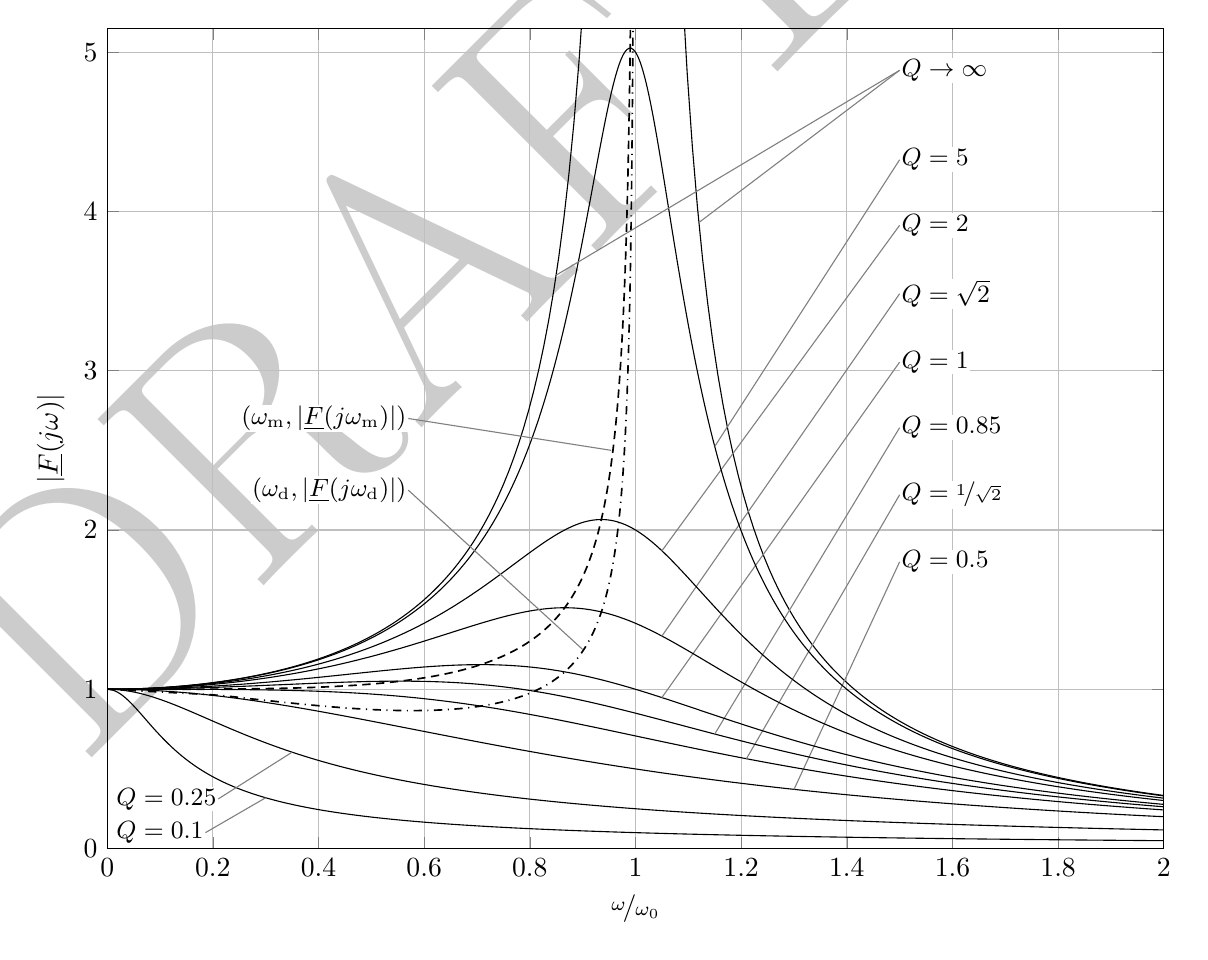
\begin{tikzpicture}
    \begin{axis}[ xlabel=$\nicefrac{\omega}{\omega_0}$
                , xmin=0
                , xmax=2
                , ymin=0
                , ymax=5.15
                , ylabel=$\left|\underline{F}(j\omega)\right|$
                , grid=major
                , ytick={0,1,...,5}
                , height=12cm
                , width=15cm
                ]

      \addplot [  draw=black
                , domain=0:0.95
                , samples=101
                ]
                {1/sqrt((1-x^2)^2)};

      \addplot [  draw=black
                , domain=1.03:2
                , samples=101
                ]
                {1/sqrt((1-x^2)^2)};

      \addplot [  draw=black
                , domain=0.71:5.5
                , samples=501
                , smooth
                , densely dashed
                , semithick
                ]
                ({sqrt(1-1/2/x^2)},{2*x^2/sqrt(4*x^2-1)});

      \addplot [  draw=black
                , domain=0.5:5.5
                , samples=501
                , smooth
                , dash dot
                , semithick
                ]
                ({sqrt(1-1/4/x^2)},{4*x^2/sqrt(16*x^2-3)});

      %Q=0.1
      \addplot [  draw=black
                , domain=0:2
                , samples=501
                , smooth
                ]
                {1/sqrt((1-x^2)^2+x^2/0.1^2)};

    \node[font=\small,fill=white,inner sep=0.5pt] (q01) 
      at (axis cs:0.1,0.1) {$Q=0.1$};
    \draw[thin,gray] (q01.east) -- (axis cs:0.3,0.319);

      %Q=0.25
      \addplot [  draw=black
                , domain=0:2
                , samples=501
                , smooth
                ]
                {1/sqrt((1-x^2)^2+x^2/0.25^2)};

    \node[font=\small,fill=white,inner sep=0.5pt,anchor=south west] (q025) 
      at ($(q01.north west) + (0,0.05)$) {$Q=0.25$};
    \draw[thin,gray] (q025.east) -- (axis cs:0.35,0.605);

      %Q=0.5
      \addplot [  draw=black
                , domain=0:2
                , samples=501
                , smooth
                ]
                {1/sqrt((1-x^2)^2+x^2/0.5^2)};
    \node[font=\small,fill=white,inner sep=0.5pt,anchor=west] (q05) 
      at (axis cs:1.5,1.8) {$Q=0.5$};
    \draw[thin,gray] (q05.west) -- (axis cs:1.3,0.371);

      %Q=1/sqrt(2)
      \addplot [  draw=black
                , domain=0:2
                , samples=501
                , smooth
                ]
                {1/sqrt((1-x^2)^2+x^2*2)};

    \node[font=\small,fill=white,inner sep=0.5pt,anchor=south west] (q0707) 
      at ($(q05.north west) + (0,0.25)$) {$Q=\nicefrac{1}{\sqrt{2}}$};
    \draw[thin,gray] (q0707.west) -- (axis cs:1.21,0.564);

      %Q=0.85
      \addplot [  draw=black
                , domain=0:2
                , samples=501
                , smooth
                ]
                {1/sqrt((1-x^2)^2+x^2/0.85^2)};

    \node[font=\small,fill=white,inner sep=0.5pt,anchor=south west] (q085) 
      at ($(q0707.north west) + (0,0.25)$) {$Q=0.85$};
    \draw[thin,gray] (q085.west) -- (axis cs:1.15,0.719);

       %Q=1
      \addplot [  draw=black
                , domain=0:2.5
                , samples=501
                , smooth
                ]
                {1/sqrt((1-x^2)^2+x^2/1^2)};

    \node[font=\small,fill=white,inner sep=0.5pt,anchor=south west] (q1) 
      at ($(q085.north west) + (0,0.25)$) {$Q=1$};
    \draw[thin,gray] (q1.west) -- (axis cs:1.05,0.948);

       %Q=sqrt(2)
      \addplot [  draw=black
                , domain=0:2.5
                , samples=501
                , smooth
                ]
                {1/sqrt((1-x^2)^2+x^2/2)};

    \node[font=\small,fill=white,inner sep=0.5pt,anchor=south west] (q141) 
      at ($(q1.north west) + (0,0.25)$) {$Q=\sqrt{2}$};
    \draw[thin,gray] (q141.west) -- (axis cs:1.05,1.334);

       %Q=2
      \addplot [  draw=black
                , domain=0:2
                , samples=501
                , smooth
                ]
                {1/sqrt((1-x^2)^2+x^2/2^2)};

    \node[font=\small,fill=white,inner sep=0.5pt,anchor=south west] (q2) 
      at ($(q141.north west) + (0,0.25)$) {$Q=2$};
    \draw[thin,gray] (q2.west) -- (axis cs:1.05,1.869);

      %Q=5
      \addplot [  draw=black
                , domain=0:2
                , samples=501
                , smooth
                ]
                {1/sqrt((1-x^2)^2+x^2/5^2)};

    \node[font=\small,fill=white,inner sep=0.5pt,anchor=south west] (q5) 
      at ($(q2.north west) + (0,0.25)$) {$Q=5$};
    \draw[thin,gray] (q5.west) -- (axis cs:1.15,2.524);

    \node[font=\small,fill=white,inner sep=0.5pt,anchor=south west] (qinfty) 
      at ($(q5.north west) + (0,0.4)$) {$Q \rightarrow \infty$};
    \draw[thin,gray] (qinfty.west) -- (axis cs:1.12,3.93);
    \draw[thin,gray] (qinfty.west) -- (axis cs:0.85,3.6);

    \node[font=\small,fill=white,inner sep=0.5pt,anchor=east] (wm) 
      at (axis cs: 0.57,2.7) 
      {$(\omega_{\mathrm{m}}, \left|\underline{F}(j\omega_{\mathrm{m}})\right|)$};
    \draw[thin,gray] (wm.east) -- (axis cs:0.954,2.5);

    \node[font=\small,fill=white,inner sep=0.5pt,anchor=east] (wr) 
      at (axis cs: 0.57,2.25) 
      {$(\omega_{\mathrm{d}}, \left|\underline{F}(j\omega_{\mathrm{d}})\right|)$};
    \draw[thin,gray] (wr.east) -- (axis cs:0.9,1.25);
    \end{axis}
  \end{tikzpicture}
  \caption{Steady-state solution $\left|\underline{F}(j\omega)\right|$ vs. normalized 
    frequency $\nicefrac{\omega}{\omega_0}$ for different qualities $Q$ and loci 
    of $(\omega_{\mathrm{m}}, \left|\underline{F}(j\omega_{\mathrm{m}})\right|)$
    and $(\omega_{\mathrm{r}}, \left|\underline{F}(j\omega_{\mathrm{r}})\right|)$}
  \label{fig:plot-fs}
\end{figure}

$\left|\underline{F}(s)\right|$ has a maximum at 
\begin{equation}
\omega_{\mathrm{m}}=
\begin{cases}
0 & \mathrm{when} \ Q <\frac{1}{\sqrt{2}} \\
\omega_0 \sqrt{1-\frac{1}{2Q^2}} & \mathrm{when} \ Q\geq\frac{1}{\sqrt{2}} \\
\end{cases} 
\end{equation}
and
\begin{equation}
\left|\underline{F}(j\omega_{\mathrm{m}})\right| =
\begin{cases}
1 & \mathrm{when} \ Q <\frac{1}{\sqrt{2}} \\
\frac{2 Q^2}{\sqrt{4Q^2-1}} & \mathrm{when} \ Q\geq\frac{1}{\sqrt{2}}. \\
\end{cases} 
\end{equation}
It is obvious that $\left|\underline{F}(j\omega_{\mathrm{m}})\right| \approx Q$
for $Q \gg 1$.
The locus $(\omega_{\mathrm{m}}, \left|\underline{F}(j\omega_{\mathrm{m}})\right|)$
is shown in Fig.~\ref{fig:plot-fs} (dashed line).
We refer to $\omega_{\mathrm{m}}$ when $Q\geq\nicefrac{1}{\sqrt{2}}$%
\footnote{The case $Q = \nicefrac{1}{\sqrt{2}}$  results
in a Butterworth filter response 
(conf. subsection \ref{subsec:examples:butterworth}).}
as resonant frequent $\omega_{\mathrm{r}}$.

\medskip

The poles of $\underline{F}(s)$ are
\begin{equation}\label{eq:poles}
p_{1,2} = - \zeta \omega_0 \pm \omega_0 \sqrt{\zeta^2-1} = - \alpha \pm \omega_0 \sqrt{\zeta^2-1}.
\end{equation}

\medskip

For $0<\zeta < 1$ (conf. Tab. \ref{tab:pz}), we transform \eqref{eq:poles} to
\begin{equation}\label{eq:poles-underdamped}
p_{1,2} = - \alpha \pm j \omega_{\mathrm{d}},
\end{equation}
with the damped oscillating frequency 
\begin{equation}\label{eq:poles}
\omega_{\mathrm{d}} = \omega_0 \sqrt{1-\zeta^2} = \omega_0 \sqrt{1-\frac{1}{4 Q^2}}
\end{equation}
and
\begin{equation}
\left|\underline{F}(j\omega_{\mathrm{d}})\right| = \frac{4 Q^2}{\sqrt{16 Q^2 -3}}.
\end{equation}

Tab.~\ref{tab:char-fs} summarizes some interesting values of
$\underline{F}(j\omega)$.
\begin{table}[H]
\centering
\caption{Characteristics of steady-state solution 
  $\left|\underline{F}(j\omega)\right|$ for different $Q$}
\begin{tabular}{cccccc}
\toprule
$Q$                      & $\zeta$                   & $\nicefrac{\omega_{\mathrm{r}}}{\omega_0}$ & $\left|\nicefrac{\underline{F}(\omega_{\mathrm{r}})}{\underline{F}(\omega_{\mathrm{0}})}\right|$ & $\nicefrac{\omega_{\mathrm{d}}}{\omega_0}$ & $\left|\nicefrac{\underline{F}(\omega_{\mathrm{d}})}{\underline{F}(\omega_{\mathrm{0}})}\right|$ \\ \midrule
0.1                      & 5                         & -                                          & -                                                                                                & -                                          & -                                                                                                \\
0.25                     & 2                         & -                                          & -                                                                                                & -                                          & -                                                                                                \\ 
0.5                      & 1                         & -                                          & -                                                                                                & 0                                          & 2                                                                                                \\
$\nicefrac{1}{\sqrt{3}}$ & $\nicefrac{\sqrt{3}}{2}$  & -                                          & -                                                                                                & 0.5                                        & 1.512                                                                                            \\ 
$\nicefrac{1}{\sqrt{2}}$ & $\nicefrac{1}{\sqrt{2}}$  & 0                                          & $\sqrt{2}$                                                                                       & $\nicefrac{1}{\sqrt{2}}$                   & 1.265                                                                                            \\
0.85                     & 0.588                     & 0.555                                      & 1.237                                                                                            & 0.809                                      & 1.162                                                                                            \\  
1                        & 0.5                       & $\nicefrac{1}{\sqrt{2}}$                   & 1.155                                                                                            & $\nicefrac{\sqrt{3}}{2}$                   & 1.109                                                                                            \\  
$\sqrt{2}$               & 0.354                     & $\nicefrac{\sqrt{3}}{2}$                   & 1.069                                                                                            & 0.935                                      & 1.05                                                                                             \\
2                        & 0.25                      & 0.935                                      & 1.033                                                                                            & 0.968                                      & 1.024                                                                                            \\ 
5                        & 0.1                       & 0.99                                       & 1.005                                                                                            & 0.995                                      & 1.004                                                                                            \\ 
$\infty$                 & 0                         & 1                                          & 1                                                                                                & 1                                          & 1                                                                                                \\ \toprule
\end{tabular}
\label{tab:char-fs}
\end{table}

Depending on $Q$, we can define four different cases. 
They are depicted in Tab.~\ref{tab:pz}.

\begin{table}[H]
  \centering
  \caption{Poles of $\underline{F}(s)$}
  \begin{tabular}{ccccc}
  \toprule
                           & \textbf{Overdamped}               & \textbf{Critically damped} & \textbf{Underdamped}                    & \textbf{Undamped}     \\ \midrule
  $Q$                       & $\left(0, \nicefrac{1}{2}\right)$ & $\nicefrac{1}{2}$          & $\left(\nicefrac{1}{2}, \infty\right)$ & $\rightarrow \infty$  \\ 
  $\zeta$                   & $\left(1, \infty\right)$          & $1$                        & $\left(0, 1\right)$                    & $0$                   \\ \hline
  $p_{1,2}$                 & $\neq$                            & $=$                        & complex conj.                          & complex conj.         \\
  $\Re\left(p_{1,2}\right)$ & $<0$                              & $<0$                       & $<0$                                   & $=0$                  \\
  $\Im\left(p_{1,2}\right)$ & $=0$                              & $=0$                       & $\neq0$                                & $\neq0$               \\
  Plot                      & \ref{fig:pz:overdamped}           & \ref{fig:pz:critdamped}    & \ref{fig:pz:underdamped}               & \ref{fig:pz:undamped} \\ \toprule
  \end{tabular}
  \label{tab:pz}
\end{table}

\begin{figure}[H]
  \centering
  \begin{subfigure}[b]{0.475\textwidth}
    \centering
    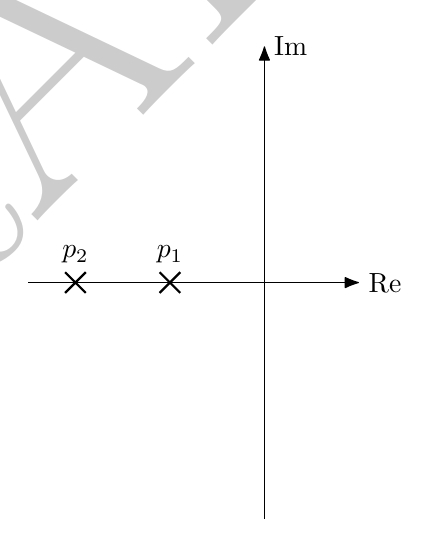
\begin{tikzpicture}[scale=1.2]
      \draw[-{Latex[round,scale=1.2,round]}] (-2.5,0) -- (1,0);
      \node[anchor=west] at (1,0) {Re};
      \draw[-{Latex[round,scale=1.2,round]}] (0,-2.5) -- (0,2.5);
      \node[anchor=west] at (0,2.5) {Im};

      \node[cross out,draw=black,thick] at (-2, 0) {};
      \node[cross out,draw=black,thick] at (-1, 0) {};
      \node[anchor=south] at (-2, 0.1) {$p_2$};
      \node[anchor=south] at (-1, 0.1) {$p_1$};
    \end{tikzpicture}
    \caption{Overdamped}
    \label{fig:pz:overdamped}
  \end{subfigure}%
  \hfill
  \begin{subfigure}[b]{0.475\textwidth}
    \centering
    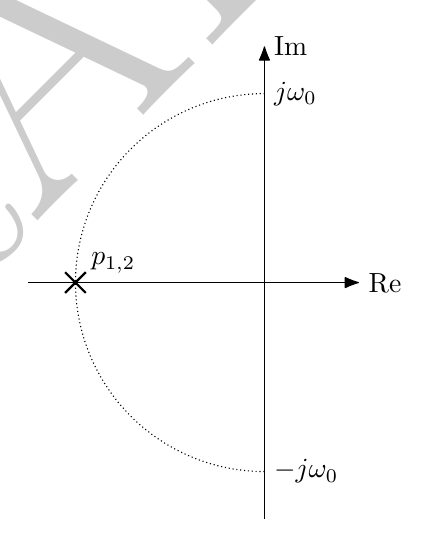
\begin{tikzpicture}[scale=1.2]
      \draw[densely dotted] plot[smooth,domain=180:360, samples=501] 
        ({2*sin(\x)},{2*cos(\x)});
      \draw[-{Latex[round,scale=1.2,round]}] (-2.5,0) -- (1,0);
      \node[anchor=west] at (1,0) {Re};
      \draw[-{Latex[round,scale=1.2,round]}] (0,-2.5) -- (0,2.5);
      \node[anchor=west] at (0,2.5) {Im};
      \node[anchor=west] at (0, 2) {$ j \omega_0$};
      \node[anchor=west] at (0,-2) {$-j \omega_0$};

      \node[cross out,draw=black,thick] at (-2, 0) {};
      \node[anchor=south] at (-1.6, 0) {$p_{1,2}$};
    \end{tikzpicture}
    \caption{Critically damped}
    \label{fig:pz:critdamped}
  \end{subfigure}
  \vskip\baselineskip
  \begin{subfigure}[b]{0.475\textwidth}
    \centering
    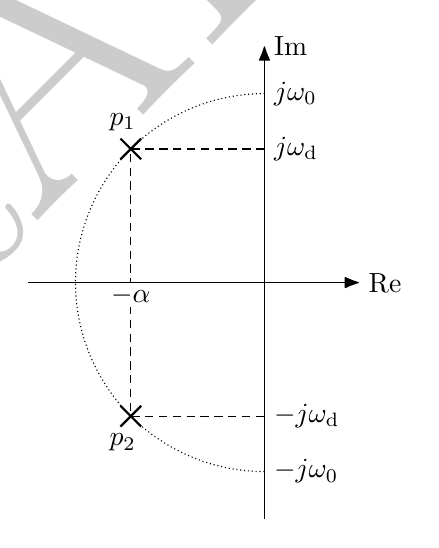
\begin{tikzpicture}[scale=1.2]
      \draw[densely dotted] plot[smooth,domain=180:360, samples=501] 
        ({2*sin(\x)},{2*cos(\x)});

      \draw[-{Latex[round,scale=1.2,round]}] (-2.5,0) -- (1,0);
      \node[anchor=west] at (1,0) {Re};
      \draw[-{Latex[round,scale=1.2,round]}] (0,-2.5) -- (0,2.5);
      \node[anchor=west] at (0,2.5) {Im};

      \node[cross out,draw=black,thick] at (-1.414,  1.414) {};
      \node[cross out,draw=black,thick] at (-1.414, -1.414) {};
      \node[anchor=south] at (-1.5, 1.5) {$p_1$};
      \node[anchor=north] at (-1.5,-1.5) {$p_2$};

      \draw[densely dashed] (0, 1.414) -- (-1.414, 1.414) -- 
                            (-1.414, -1.414) -- (0, -1.414);

      \node[anchor=west] at (0, 2) {$ j \omega_0$};
      \node[anchor=west] at (0,-2) {$-j \omega_0$};

      \node[anchor=west] at (0, 1.414) {$ j \omega_{\mathrm{d}}$};
      \node[anchor=west] at (0,-1.414) {$-j \omega_{\mathrm{d}}$};

      \node[anchor=north,fill=white,inner sep=1pt] at (-1.414,0) {$-\alpha$};
    \end{tikzpicture}
    \caption{Underdamped}
    \label{fig:pz:underdamped}
  \end{subfigure}%
  \hfill
  \begin{subfigure}[b]{0.475\textwidth}
    \centering
    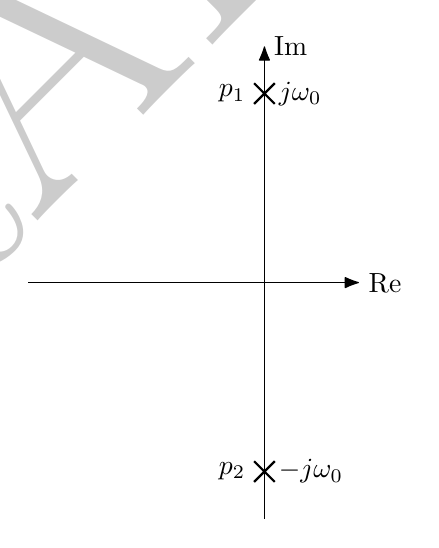
\begin{tikzpicture}[scale=1.2]
      \draw[-{Latex[round,scale=1.2,round]}] (-2.5,0) -- (1,0);
      \node[anchor=west] at (1,0) {Re};
      \draw[-{Latex[round,scale=1.2,round]}] (0,-2.5) -- (0,2.5);
      \node[anchor=west] at (0,2.5) {Im};

      \node[cross out,draw=black,thick] at (0,  2) {};
      \node[cross out,draw=black,thick] at (0, -2) {};
      \node[anchor=east] at (-0.1, 2) {$p_1$};
      \node[anchor=east] at (-0.1,-2) {$p_2$};

      \node[anchor=west] at (0.05, 2) {$ j \omega_0$};
      \node[anchor=west] at (0.05,-2) {$-j \omega_0$};
    \end{tikzpicture}
    \caption{Undamped}
    \label{fig:pz:undamped}
  \end{subfigure}
  \caption{Pole-zero plot}
  \label{fig:squarelawtransf}
\end{figure}

\section{Step Response}

\begin{equation}
x(t) =
\begin{cases}
0 & \mathrm{when} \ t < 0    \\
1 & \mathrm{when} \ t \geq 0 \\
\end{cases} 
\end{equation}

\begin{equation}
 T_0 = \frac{2\pi}{\omega_0}
\end{equation}

\begin{equation}
 T_{\mathrm{d}} = \frac{2\pi}{\omega_d} 
                = \frac{2\pi}{\omega_0 \sqrt{1-\zeta^2}}
                = \frac{T_0}{\sqrt{1-\zeta^2}} 
                = \frac{T_0}{\sqrt{1-\frac{1}{4 Q^2}}}                 
\end{equation}

\begin{equation}
y(t)=
\begin{cases}
-                                  & \mathrm{when} \ Q <\frac{1}{2} \\
1 - e^{-\omega_0 t} (1+\omega_0 t) & \mathrm{when} \ Q = \frac{1}{2} \\
-                                  & \mathrm{when} \ \frac{1}{2} < Q  \\
1 - \cos(\omega_0 t)               & \mathrm{when} \  Q \rightarrow \infty \\
\end{cases} 
\end{equation}

\begin{equation}
y'(0)=
\begin{cases}
-        & \mathrm{when} \ Q <\frac{1}{2} \\
\omega_0 & \mathrm{when} \ Q = \frac{1}{2} \\
-        & \mathrm{when} \ \frac{1}{2} < Q  \\
0        & \mathrm{when} \  Q \rightarrow \infty \\
\end{cases} 
\end{equation}


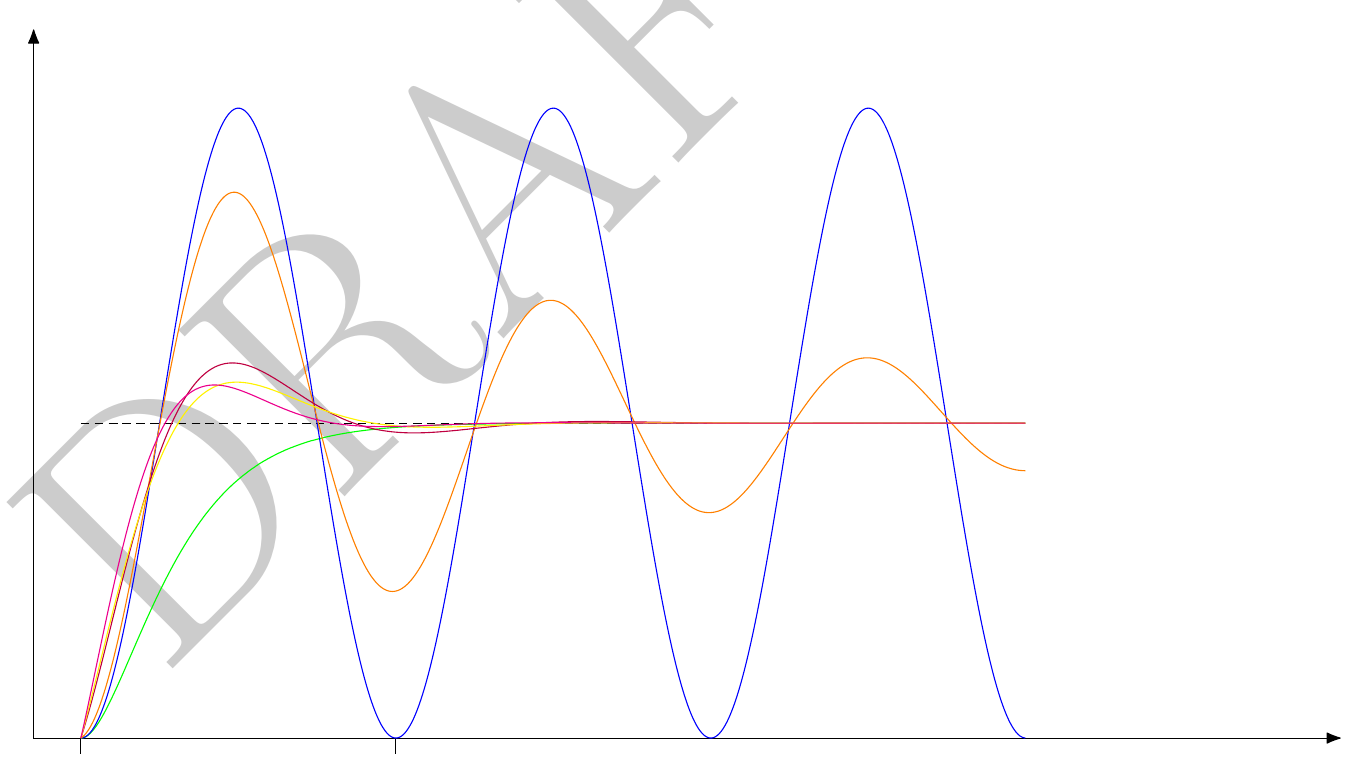
\begin{tikzpicture}[scale=4]
  \draw[{Latex[round,scale=1.2,round]}-{Latex[round,scale=1.2,round]}] 
    (-0.15,2.25) -- (-0.15,0) -- (4,0);
  \draw (0,0) -- (0,-0.05);
  \draw (1,0) -- (1,-0.05);

  \draw[densely dashed] plot[smooth,domain=0:3, samples=501] 
    ({\x},{1});

  \draw[green] plot[smooth,domain=0:3, samples=501] 
    ({\x},{1-e^(-2*pi*\x)*(1+2*pi*\x)});

  %\draw[red] plot[smooth,domain=0:4, samples=501] 
  %  ({\x},{1-e^(-\x)*(1+\x)});

  \draw[blue] plot[smooth,domain=0:3, samples=501] 
    ({\x},{1-cos(360*\x)});

  \draw[orange] plot[smooth,domain=0:3, samples=501] 
    ({\x},{1-e^(-pi/5*\x)*cos(sqrt(1-1/4/(5)^2)*360*\x)});

  \draw[purple] plot[smooth,domain=0:3, samples=501] 
    ({\x},{1-e^(-pi/1*\x)*cos(sqrt(1-1/4/(1)^2)*360*\x)});

  \draw[yellow] plot[smooth,domain=0:3, samples=501] 
    ({\x},{1-e^(-pi/0.85*\x)*cos(sqrt(1-1/4/(0.85)^2)*360*\x)});

  \draw[magenta] plot[smooth,domain=0:3, samples=501] 
    ({\x},{1-e^(-pi*sqrt(2)*\x)*cos(sqrt(1-1/4*0.5)*360*\x)});
\end{tikzpicture}



\begin{figure}[H]
  \centering
  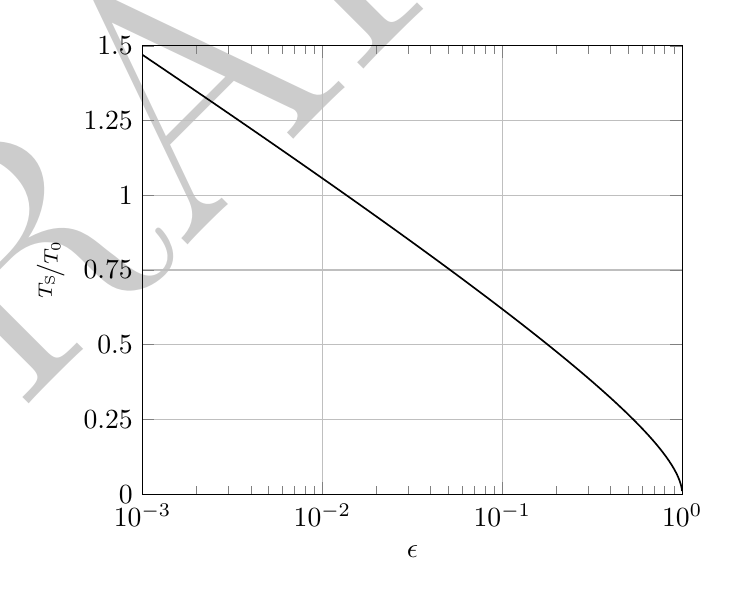
\begin{tikzpicture}
    \begin{axis}[ xlabel=$\epsilon$
                , xmin=1e-3
                , xmax=1
                , ymin=0
                , ymax=1.5
                , ylabel=$\nicefrac{T_{\mathrm{S}}}{T_{\mathrm{0}}}$
                , grid=major
                , ytick={0,0.25,...,1.5}
                , xmode=log
                ]
        \addplot [  draw=black
                  , domain=0.01:1.5
                  , samples=501
                  , smooth
                  , semithick
                  ]
                  ({e^(-2*pi*x)*(1+2*pi*x)},{x});
    \end{axis}              
  \end{tikzpicture}
  \caption{Relative settling time $\nicefrac{T_{\mathrm{S}}}{T_{\mathrm{0}}}$
    vs. deviation $\epsilon$ from final value in the critically damped case}
  \label{fig:settling-crit-damped}
\end{figure}

\section{Examples}\label{sec:examples}

\subsection{Butterworth}\label{subsec:examples:butterworth}

\begin{equation}
\underline{F}_{\mathrm{BW,2}} = \frac{\underline{Y}(s)}{\underline{X}(s)} 
                 = \frac{\omega_0^2}{s^2 + \sqrt{2} \omega_0 s + \omega_0^2 }
\end{equation}

\begin{equation}
Q_{\mathrm{BW,2}}(s) = \frac{1}{\sqrt{2}}
\end{equation}

\subsection{Bessel}
tbd
\begin{equation}
Q_{\mathrm{BS,2}}(s) = \frac{1}{\sqrt{3}}
\end{equation}
\subsection{Series RLC}

\begin{figure}[H]
  \centering
  \begin{circuitikz}
    \RlcSeriesSchematicA
  \end{circuitikz}
  \caption{Schematic of series RLC resonator}
  \label{fig:series-res}
\end{figure}

\begin{equation}\label{eq:rlc-series:fs}
\underline{F}(s) = \frac{\underline{V}_{\mathrm{O}}(s)}{\underline{V}_{\mathrm{I}}(s)} 
                 = \frac{\frac{1}{sC}}{R+sL+\frac{1}{sC}}
                 = \frac{1}{1 + sRC+s^2LC}
                 = \frac{\frac{1}{LC}}{s^2+s \frac{R}{L} + \frac{1}{LC}}                 
\end{equation}

A coefficient comparison between \eqref{eq:rlc-series:fs} and \eqref{eq:fs}
results in 
\begin{equation}
\omega_0 = \frac{1}{\sqrt{LC}}
\end{equation}
and
\begin{equation}
Q = \frac{L}{R} \omega_0 = \frac{1}{R} \sqrt{\frac{L}{C}}.
\end{equation}

\begin{equation}
Q = \frac{X}{R} = \frac{1}{\omega_0 R C} = \frac{\omega_0 L}{R}
\end{equation}

\subsection{Parallel RLC}
tbd
\end{document}